\paragraph{QuizziPedia::Front-End::Controllers::LangController}
\begin{figure} [ht]
	\centering
	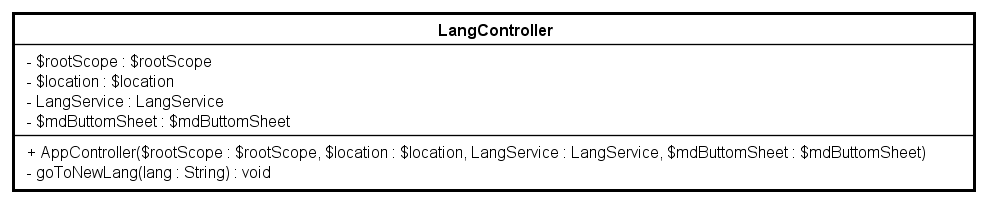
\includegraphics[scale=0.5]{UML/Classi/Front-End/QuizziPedia_Front-end_Controller_LangController.png}
	\caption{QuizziPedia::Front-End::Controllers::LangController}
\end{figure} \FloatBarrier
\begin{itemize}
	\item \textbf{Descrizione}: questa classe permette di ottenere un nuovo set di variabili per la nuova traduzione dell'applicazione;
	\item \textbf{Utilizzo}: fornisce le funzionalità per cambiare la lingua del sistema;
	\item \textbf{Relazione con altre classi}:
	\begin{itemize}
		\item \textbf{IN \texttt{AppController}}: questa classe permette di gestire per ogni pagina dell'applicazione l'autenticazione e l'autorizzazione dell'utente che si posiziona in essa e mostrare la lingua corretta;
		\item \textbf{IN \texttt{MenuBarController}}: questa classe permette di gestire il menù fisso per ogni pagina.
	\end{itemize}
	\item \textbf{Attributi}:
	\begin{itemize}
		\item \texttt{-} \texttt{\$rootScope: \$rootScope} \\
		Campo dati contenente il riferimento all'oggetto globale \$rootScope creato da \textit{Angular\ped{G}}. Viene utilizzato per rendere accessibile a tutti i \textit{controller\ped{G}} e a tutte le \textit{view\ped{G}} l'oggetto \texttt{UserDetailsModel}. In questo caso viene utilizzato per inserire in \$rootScope l'oggetto di ritorno della chiamata a \texttt{getUserDetails} del \textit{service\ped{G}} \texttt{UserDetailsService};
		\item \texttt{-} \texttt{\$location: \$location} \\
		Campo dati contenente un riferimento al servizio creato da \textit{Angular\ped{G}} che permette di accedere alla barra degli indirizzi del \textit{browser\ped{G}}, i cambiamenti all'URL nella barra degli indirizzi si riflettono in questo oggetto e viceversa; 
		\item \texttt{-} \texttt{LangService: LangService} \\
		Campo dati contenente un riferimento alla classe che permette di gestire la lingua nella quale si è scelto di utilizzare l'applicazione;
		\item \texttt{-} \texttt{\$mdBottomSheet: \$mdBottomSheet}: \\
		Servizio offerto dalla libreria \texttt{Angular Material} che permette di aprire una tendina a scorrimento sopra la vista principale per mostrare un set di bottoni. Implementa le \texttt{promise}. In \textit{QuizziPedia} serve per poter scegliere la lingua con sui visualizzare l'applicazione.
	\end{itemize}	
		\item \textbf{Metodi}:
		\begin{itemize}
		\item \texttt{+} \texttt{LangController(\$rootScope: \$rootScope, \$location: \$location, LangService: LangService, \$mdBottomSheet: \$mdBottomSheet)} \\ Metodo costruttore della classe.\\
		\textbf{Parametri}: 
		\begin{itemize}
			\item \texttt{\$rootScope: \$rootScope} \\
			Parametro contenente il riferimento all'oggetto globale \$rootScope creato da \textit{An-\\gular\ped{G}}. Viene utilizzato per rendere accessibile a tutti i \textit{controller\ped{G}} e a tutte le \textit{view\ped{G}} l'oggetto \texttt{UserDetailsModel}. In questo caso viene utilizzato per inserire in \$rootScope l'oggetto di ritorno della chiamata a \texttt{getUserDetails} del \textit{service\ped{G}} \texttt{UserDetai-\\lsService};
			\item \texttt{-} \texttt{\$location: \$location} \\
			Parametro contenente un riferimento al servizio creato da \textit{Angular\ped{G}} che permette di accedere alla barra degli indirizzi del \textit{browser\ped{G}}, i cambiamenti all'URL nella barra degli indirizzi si riflettono in questo oggetto e viceversa; 
			\item \texttt{LangService: LangService} \\
			Parametro contenente un riferimento alla classe che permette di gestire la lingua nella quale si è scelto di utilizzare l'applicazione;
			\item \texttt{\$mdBottomSheet: \$mdBottomSheet}: \\
			Parametro contenente un riferimento al servizio offerto dalla libreria \texttt{Angular Material} che permette di aprire una tendina a scorrimento sopra la vista principale per mostrare un set di bottoni. Implementa le \texttt{promise}. In \textit{QuizziPedia} serve per poter scegliere la lingua con sui visualizzare l'applicazione.
		\end{itemize}
		\item \texttt{-} \texttt{goToNewLang(lang: String): void} \\ Metodo che permette di cambiare lingua al sistema con una chiamata a \texttt{LangService}.\\
		\textbf{Parametri}:
		\begin{itemize}
			\item \texttt{lang: String}: parametro che identifica la lingua del sistema.
		\end{itemize}
	
	\end{itemize}
\end{itemize}

